% !TEX TS-program = lualatex
% !TEX encoding = UTF-8 Unicode
\documentclass[12pt,a4paper]{article}

\IfFileExists{src/libs/body.tex}{% --- body.tex ---
\usepackage{pdfpages}
\usepackage{fontspec}
% Prefer Times New Roman when available; fall back in container environments.
\IfFontExistsTF{Times New Roman}{
  \setmainfont{Times New Roman}
}{
  \setmainfont{Liberation Serif}
}
\usepackage[vietnamese]{babel}

% Page layout and spacing
\usepackage[left=3cm,right=2cm,top=2cm,bottom=2cm]{geometry}
\usepackage{titlesec}
\usepackage{setspace}

% Silence noisy warnings
\usepackage{silence}
\WarningFilter{transparent}{Loading aborted}
\WarningFilter{hyperref}{The anchor of a bookmark and its parent's}

% Core packages
\usepackage{float}
\usepackage{svg}
\usepackage{graphicx}
\graphicspath{{assets/}{../assets/}{../../assets/}}
\svgpath{{assets/}{../assets/}{../../assets/}}
\usepackage{enumitem}
\usepackage{array}
\usepackage{tabularx}
\usepackage{multirow}
\usepackage[table]{xcolor}
\usepackage{ulem}
\usepackage{xurl}

% ====== THÊM 2 GÓI NÀY ĐỂ FIX LỖI ADJUSTBOX VÀ FOREST ======
\usepackage{adjustbox}
\usepackage[edges]{forest}
% ============================================================

% TikZ
\usepackage{tikz}

% ====== BỔ SUNG FIT, BACKGROUNDS, TREES VÀO DANH SÁCH ======
\usetikzlibrary{calc, arrows.meta, shapes.geometric, positioning, fit, backgrounds, trees}

% Table tuning
\renewcommand{\tabularxcolumn}[1]{m{#1}}
\hbadness=10000
\hfuzz=10000pt

% Shared commands
\newcommand{\subsecheading}[1]{%
    \par\vspace{2pt}%
    \hspace{1.5em}\textbf{#1}%
    \par\vspace{2pt}%
}
\newcommand{\introtext}[1]{%
    \par\hspace{3.0em}#1\par%
}
\newcommand{\StandaloneDocumentSetup}[2]{%
  \pagenumbering{arabic}%
  \ApplyStandardFooter{#1}{#2}%
}
\newcommand{\StandaloneSectionSetup}[2]{%
  \ApplyStandardFooter{#1}{#2}%
}

% Math
\usepackage{amsmath}

% Hyperref
\usepackage{hyperref}
\hypersetup{
    colorlinks=true,
    linkcolor=black,
    filecolor=magenta,
    urlcolor=blue,
}}{%
  \IfFileExists{../libs/body.tex}{% --- body.tex ---
\usepackage{pdfpages}
\usepackage{fontspec}
% Prefer Times New Roman when available; fall back in container environments.
\IfFontExistsTF{Times New Roman}{
  \setmainfont{Times New Roman}
}{
  \setmainfont{Liberation Serif}
}
\usepackage[vietnamese]{babel}

% Page layout and spacing
\usepackage[left=3cm,right=2cm,top=2cm,bottom=2cm]{geometry}
\usepackage{titlesec}
\usepackage{setspace}

% Silence noisy warnings
\usepackage{silence}
\WarningFilter{transparent}{Loading aborted}
\WarningFilter{hyperref}{The anchor of a bookmark and its parent's}

% Core packages
\usepackage{float}
\usepackage{svg}
\usepackage{graphicx}
\graphicspath{{assets/}{../assets/}{../../assets/}}
\svgpath{{assets/}{../assets/}{../../assets/}}
\usepackage{enumitem}
\usepackage{array}
\usepackage{tabularx}
\usepackage{multirow}
\usepackage[table]{xcolor}
\usepackage{ulem}
\usepackage{xurl}

% ====== THÊM 2 GÓI NÀY ĐỂ FIX LỖI ADJUSTBOX VÀ FOREST ======
\usepackage{adjustbox}
\usepackage[edges]{forest}
% ============================================================

% TikZ
\usepackage{tikz}

% ====== BỔ SUNG FIT, BACKGROUNDS, TREES VÀO DANH SÁCH ======
\usetikzlibrary{calc, arrows.meta, shapes.geometric, positioning, fit, backgrounds, trees}

% Table tuning
\renewcommand{\tabularxcolumn}[1]{m{#1}}
\hbadness=10000
\hfuzz=10000pt

% Shared commands
\newcommand{\subsecheading}[1]{%
    \par\vspace{2pt}%
    \hspace{1.5em}\textbf{#1}%
    \par\vspace{2pt}%
}
\newcommand{\introtext}[1]{%
    \par\hspace{3.0em}#1\par%
}
\newcommand{\StandaloneDocumentSetup}[2]{%
  \pagenumbering{arabic}%
  \ApplyStandardFooter{#1}{#2}%
}
\newcommand{\StandaloneSectionSetup}[2]{%
  \ApplyStandardFooter{#1}{#2}%
}

% Math
\usepackage{amsmath}

% Hyperref
\usepackage{hyperref}
\hypersetup{
    colorlinks=true,
    linkcolor=black,
    filecolor=magenta,
    urlcolor=blue,
}}{% --- body.tex ---
\usepackage{pdfpages}
\usepackage{fontspec}
% Prefer Times New Roman when available; fall back in container environments.
\IfFontExistsTF{Times New Roman}{
  \setmainfont{Times New Roman}
}{
  \setmainfont{Liberation Serif}
}
\usepackage[vietnamese]{babel}

% Page layout and spacing
\usepackage[left=3cm,right=2cm,top=2cm,bottom=2cm]{geometry}
\usepackage{titlesec}
\usepackage{setspace}

% Silence noisy warnings
\usepackage{silence}
\WarningFilter{transparent}{Loading aborted}
\WarningFilter{hyperref}{The anchor of a bookmark and its parent's}

% Core packages
\usepackage{float}
\usepackage{svg}
\usepackage{graphicx}
\graphicspath{{assets/}{../assets/}{../../assets/}}
\svgpath{{assets/}{../assets/}{../../assets/}}
\usepackage{enumitem}
\usepackage{array}
\usepackage{tabularx}
\usepackage{multirow}
\usepackage[table]{xcolor}
\usepackage{ulem}
\usepackage{xurl}

% ====== THÊM 2 GÓI NÀY ĐỂ FIX LỖI ADJUSTBOX VÀ FOREST ======
\usepackage{adjustbox}
\usepackage[edges]{forest}
% ============================================================

% TikZ
\usepackage{tikz}

% ====== BỔ SUNG FIT, BACKGROUNDS, TREES VÀO DANH SÁCH ======
\usetikzlibrary{calc, arrows.meta, shapes.geometric, positioning, fit, backgrounds, trees}

% Table tuning
\renewcommand{\tabularxcolumn}[1]{m{#1}}
\hbadness=10000
\hfuzz=10000pt

% Shared commands
\newcommand{\subsecheading}[1]{%
    \par\vspace{2pt}%
    \hspace{1.5em}\textbf{#1}%
    \par\vspace{2pt}%
}
\newcommand{\introtext}[1]{%
    \par\hspace{3.0em}#1\par%
}
\newcommand{\StandaloneDocumentSetup}[2]{%
  \pagenumbering{arabic}%
  \ApplyStandardFooter{#1}{#2}%
}
\newcommand{\StandaloneSectionSetup}[2]{%
  \ApplyStandardFooter{#1}{#2}%
}

% Math
\usepackage{amsmath}

% Hyperref
\usepackage{hyperref}
\hypersetup{
    colorlinks=true,
    linkcolor=black,
    filecolor=magenta,
    urlcolor=blue,
}}%
}
\IfFileExists{src/libs/header.tex}{% --- header.tex ---
\usepackage{fancyhdr}
\setlength{\headheight}{15.5pt} % Thêm dòng này để fix cảnh báo chiều cao
%\setlength{\headheight}{14.5pt}
\addtolength{\topmargin}{-2.5pt}

\pagestyle{fancy}
\fancyhf{}
\renewcommand{\headrulewidth}{0pt}
\renewcommand{\footrulewidth}{0pt}

\newcommand{\ApplyStandardHeader}{%
  \fancyhead[L]{%
    \begin{minipage}[t]{0.795\linewidth}%
      UIT \textbar{} SS004.F21 \textbar{} Nhóm 03 \textbar{} Đồ án cuối kỳ%
    \end{minipage}%
    \vrule%
    \begin{minipage}[t]{0.185\linewidth}%
      \centering cTetris%
    \end{minipage}%
  }%
}

\ApplyStandardHeader
}{%
  \IfFileExists{../libs/header.tex}{% --- header.tex ---
\usepackage{fancyhdr}
\setlength{\headheight}{15.5pt} % Thêm dòng này để fix cảnh báo chiều cao
%\setlength{\headheight}{14.5pt}
\addtolength{\topmargin}{-2.5pt}

\pagestyle{fancy}
\fancyhf{}
\renewcommand{\headrulewidth}{0pt}
\renewcommand{\footrulewidth}{0pt}

\newcommand{\ApplyStandardHeader}{%
  \fancyhead[L]{%
    \begin{minipage}[t]{0.795\linewidth}%
      UIT \textbar{} SS004.F21 \textbar{} Nhóm 03 \textbar{} Đồ án cuối kỳ%
    \end{minipage}%
    \vrule%
    \begin{minipage}[t]{0.185\linewidth}%
      \centering cTetris%
    \end{minipage}%
  }%
}

\ApplyStandardHeader
}{% --- header.tex ---
\usepackage{fancyhdr}
\setlength{\headheight}{15.5pt} % Thêm dòng này để fix cảnh báo chiều cao
%\setlength{\headheight}{14.5pt}
\addtolength{\topmargin}{-2.5pt}

\pagestyle{fancy}
\fancyhf{}
\renewcommand{\headrulewidth}{0pt}
\renewcommand{\footrulewidth}{0pt}

\newcommand{\ApplyStandardHeader}{%
  \fancyhead[L]{%
    \begin{minipage}[t]{0.795\linewidth}%
      UIT \textbar{} SS004.F21 \textbar{} Nhóm 03 \textbar{} Đồ án cuối kỳ%
    \end{minipage}%
    \vrule%
    \begin{minipage}[t]{0.185\linewidth}%
      \centering cTetris%
    \end{minipage}%
  }%
}

\ApplyStandardHeader
}%
}
\IfFileExists{src/libs/footer.tex}{% --- footer.tex ---
\usepackage{lastpage}

\newcommand{\ApplyStandardFooter}[2]{%
  \fancyfoot[L]{%
    \begin{minipage}[t]{0.795\linewidth}%
      Document ID: #1%
    \end{minipage}%
    \vrule%
    \begin{minipage}[t]{0.185\linewidth}%
      \centering\thepage/\pageref{#2}%
    \end{minipage}%
  }%
  \fancypagestyle{plain}{%
    \fancyhf{}%
    \renewcommand{\headrulewidth}{0pt}%
    \renewcommand{\footrulewidth}{0pt}%
    \ApplyStandardHeader%
    \fancyfoot[L]{%
      \begin{minipage}[t]{0.795\linewidth}%
        Document ID: #1%
      \end{minipage}%
      \vrule%
      \begin{minipage}[t]{0.185\linewidth}%
        \centering\thepage/\pageref{#2}%
      \end{minipage}%
    }%
  }%
  \pagestyle{fancy}%
}
}{%
  \IfFileExists{../libs/footer.tex}{% --- footer.tex ---
\usepackage{lastpage}

\newcommand{\ApplyStandardFooter}[2]{%
  \fancyfoot[L]{%
    \begin{minipage}[t]{0.795\linewidth}%
      Document ID: #1%
    \end{minipage}%
    \vrule%
    \begin{minipage}[t]{0.185\linewidth}%
      \centering\thepage/\pageref{#2}%
    \end{minipage}%
  }%
  \fancypagestyle{plain}{%
    \fancyhf{}%
    \renewcommand{\headrulewidth}{0pt}%
    \renewcommand{\footrulewidth}{0pt}%
    \ApplyStandardHeader%
    \fancyfoot[L]{%
      \begin{minipage}[t]{0.795\linewidth}%
        Document ID: #1%
      \end{minipage}%
      \vrule%
      \begin{minipage}[t]{0.185\linewidth}%
        \centering\thepage/\pageref{#2}%
      \end{minipage}%
    }%
  }%
  \pagestyle{fancy}%
}
}{% --- footer.tex ---
\usepackage{lastpage}

\newcommand{\ApplyStandardFooter}[2]{%
  \fancyfoot[L]{%
    \begin{minipage}[t]{0.795\linewidth}%
      Document ID: #1%
    \end{minipage}%
    \vrule%
    \begin{minipage}[t]{0.185\linewidth}%
      \centering\thepage/\pageref{#2}%
    \end{minipage}%
  }%
  \fancypagestyle{plain}{%
    \fancyhf{}%
    \renewcommand{\headrulewidth}{0pt}%
    \renewcommand{\footrulewidth}{0pt}%
    \ApplyStandardHeader%
    \fancyfoot[L]{%
      \begin{minipage}[t]{0.795\linewidth}%
        Document ID: #1%
      \end{minipage}%
      \vrule%
      \begin{minipage}[t]{0.185\linewidth}%
        \centering\thepage/\pageref{#2}%
      \end{minipage}%
    }%
  }%
  \pagestyle{fancy}%
}
}%
}
\usepackage{docmute}

\hypersetup{pdftitle={Hướng dẫn sử dụng tính năng cấu hình - v1 \& v2}}

% Tip/note box style cho v2
\renewcommand{\tipbox}[1]{%
  \vspace{4pt}%
  \noindent\colorbox{yellow!18}{\begin{minipage}{0.96\linewidth}%
    \vspace{2pt}\textbf{Mẹo nhanh:} #1\vspace{2pt}%
  \end{minipage}}%
  \vspace{4pt}%
}
\renewcommand{\notebox}[1]{%
  \vspace{4pt}%
  \noindent\colorbox{cyan!12}{\begin{minipage}{0.96\linewidth}%
    \vspace{2pt}\textbf{Lưu ý:} #1\vspace{2pt}%
  \end{minipage}}%
  \vspace{4pt}%
}

\begin{document}
\providecommand{\StandaloneSectionSetup}[2]{\ApplyStandardFooter{#1}{#2}}
\StandaloneSectionSetup{09-gameConsoleGuide.tex}{LastPageGameConsoleGuide}
\onehalfspacing

\section{Hướng dẫn sử dụng tính năng cấu hình (phiên bản 1)}

\subsection{Tổng quan}
\textbf{gameConsole} là \textit{hub screen} (màn hình trung tâm) của ứng dụng \textit{cTetris}.
Đây là nơi bạn khởi động ván đấu, tra cứu hướng dẫn chơi, xem bảng xếp hạng, và thoát ứng dụng.
Màn hình được thiết kế cố định theo tỉ lệ 9:16 (portrait), đảm bảo hiển thị nhất quán trên cả ứng dụng máy tính và trình duyệt web (WASM).

\noindent\textbf{Vị trí của gameConsole trong luồng ứng dụng:}
\begin{itemize}
    \item Khi mở ứng dụng, bạn lần lượt đi qua: \textit{gameStory} (màn hình mở đầu) $\rightarrow$ \textit{gameConsole} (màn hình đang đọc).
    \item Từ \textit{gameConsole}, nhấn \textbf{PLAY} để vào màn hình chơi chính (\textit{gameCore}).
    \item Từ \textit{gameCore}, nhấn nút \textit{power off} trên thanh bên rồi chọn \textbf{Console} để quay lại đây.
\end{itemize}

\begin{figure}[htbp]
    \centering
    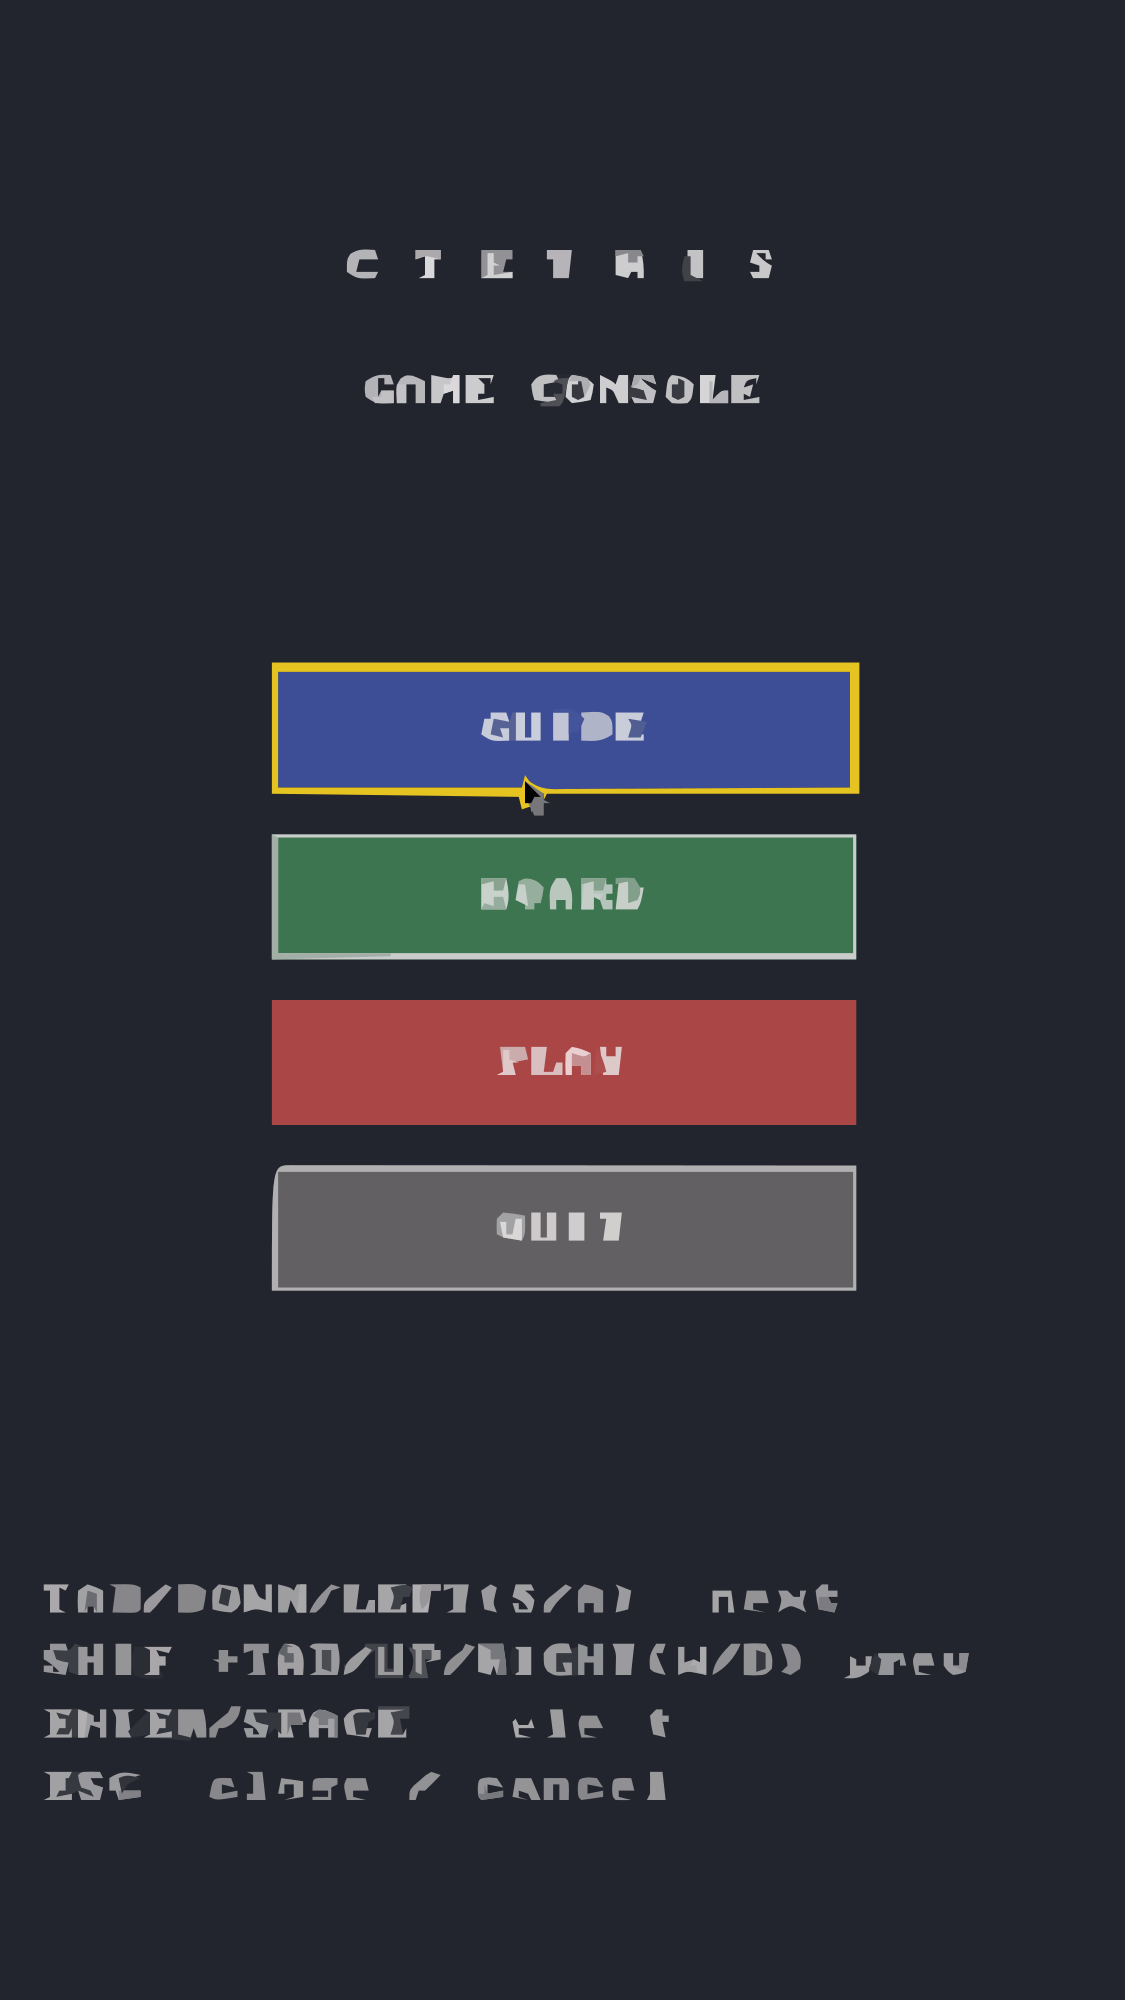
\includegraphics[width=0.3\textwidth]{09-gameConsoleGuide-screenshot}
    \\[10pt]
    \textit{\small Hình 9.1: Màn hình module gameConsole - V1}
\end{figure}

\subsection{Giao diện màn hình chính}
Màn hình chính được chia thành ba vùng theo chiều dọc:
\begin{itemize}
    \item \textbf{Vùng tiêu đề} (trên cùng) -- hiển thị tên thương hiệu \textit{C TETRIS -- GAME CONSOLE}.
    \item \textbf{Vùng nút bấm} (giữa) -- gồm 4 nút điều khiển chính, kích thước đồng nhất \texttt{140$\times$30 px}, sắp xếp dọc thẳng hàng.
    \item \textbf{Vùng phím tắt} (dưới cùng) -- hiển thị gợi ý các phím điều hướng (TAB, ENTER, ESC...) để bạn dễ nhớ khi chơi.
\end{itemize}

\noindent Nền màn hình dùng màu xám đậm \texttt{\#282C34} -- vừa đủ tối để các nút màu nổi bật, vừa dễ chịu cho mắt khi nhìn lâu.

\subsection{Bốn nút điều khiển chính}
Bốn nút bấm trung tâm là cách duy nhất để rời khỏi gameConsole.
Mỗi nút có màu sắc riêng để bạn nhận diện nhanh ngay cả khi không đọc chữ:

\vspace{4pt}
\begin{tabularx}{\linewidth}{|l|l|X|}
    \hline
    \textbf{Nút} & \textbf{Màu nền} & \textbf{Chức năng} \\
    \hline
    \textbf{GUIDE} & Xanh dương đậm & Mở popup hướng dẫn cách chơi (\textit{Guide Lightbox}). \\
    \hline
    \textbf{BOARD} & Xanh lá đậm   & Mở popup bảng xếp hạng (\textit{Leaderboard Lightbox}). \\
    \hline
    \textbf{PLAY}  & Đỏ đậm        & Chuyển sang màn hình chơi chính \textit{gameCore}. \\
    \hline
    \textbf{QUIT}  & Xám trung tính & Thoát ứng dụng. Trên web (WASM) sẽ chuyển sang màn hình \textit{Reload} thay vì đóng trực tiếp. \\
    \hline
\end{tabularx}

\vspace{4pt}
\noindent\textit{Mẹo nhận diện trạng thái:} nút đang được \textbf{focus} (chọn để kích hoạt) sẽ có \textbf{viền vàng đôi} bao quanh.
Nhờ đó, ngay cả khi không nhìn vào con trỏ chuột, bạn vẫn biết mình đang đứng ở nút nào.

\subsection{Hệ thống điều hướng}
gameConsole hỗ trợ song song ba kênh điều hướng và bạn có thể kết hợp tự do trong cùng một phiên.

\subsubsection{Điều hướng bằng bàn phím}
Hệ thống chấp nhận nhiều bộ phím tương đương để bạn dùng tay nào cũng thuận:

\vspace{4pt}
\begin{tabularx}{\linewidth}{|l|X|}
    \hline
    \textbf{Phím} & \textbf{Hành động trên màn hình chính} \\
    \hline
    \texttt{TAB} \,/\, \texttt{S} \,/\, \texttt{A}                & Chuyển focus tiến tới nút kế tiếp (theo chiều xuống). \\
    \hline
    \texttt{Shift+TAB} \,/\, \texttt{W} \,/\, \texttt{D}          & Chuyển focus lùi về nút trước đó (theo chiều lên). \\
    \hline
    \texttt{ENTER} \,/\, \texttt{SPACE}                            & Kích hoạt nút đang được focus. \\
    \hline
    \texttt{ESC}                                                    & Nhảy nhanh focus về nút \textbf{QUIT}. \\
    \hline
\end{tabularx}

\subsubsection{Điều hướng bằng chuột và con lăn}
\begin{itemize}
    \item \textbf{Click chuột trái} vào bất kỳ nút nào: kích hoạt nút đó ngay lập tức, đồng thời cập nhật focus về nút vừa click.
    \item \textbf{Click vào nút \texttt{[X]}} ở góc trên phải của popup (Guide hoặc Board): đóng popup.
    \item \textbf{Con lăn chuột} (\textit{mouse wheel}): cuộn nội dung khi popup Guide hoặc Board đang mở.
\end{itemize}

\subsection{Scrollbar tương tác}
Hai popup \textbf{GUIDE} và \textbf{BOARD} đều dùng chung một \textit{scrollbar} (thanh cuộn) đặt bên phải.
Scrollbar hỗ trợ bốn kiểu tương tác để bạn cuộn dài hay ngắn đều thuận tiện:

\vspace{4pt}
\begin{tabularx}{\linewidth}{|l|X|}
    \hline
    \textbf{Kiểu tương tác} & \textbf{Cách thực hiện} \\
    \hline
    \textbf{Kéo thả} (Drag)         & Nhấn giữ chuột lên \textit{thumb} (con trượt) và kéo theo chiều dọc. \\
    \hline
    \textbf{Click track}            & Click vào phần rãnh trống (ngoài thumb) để nhảy cóc tới vị trí tương ứng. \\
    \hline
    \textbf{Click mũi tên}          & Click vào nút ▲ hoặc ▼ ở hai đầu để cuộn từng dòng. \\
    \hline
    \textbf{Auto-repeat}            & Giữ chuột trên nút mũi tên: sau 300 ms, scrollbar tự động cuộn liên tục mỗi 60 ms. \\
    \hline
\end{tabularx}

\vspace{4pt}
\noindent\textbf{Phản hồi thị giác:}
\begin{itemize}
    \item Nút mũi tên đổi sang \textbf{màu vàng nổi bật} khi đang được nhấn giữ.
    \item Thumb chuyển sang màu vàng trong toàn bộ thời gian bạn kéo thả.
    \item Thumb \textbf{tự co dãn kích thước} theo tỉ lệ giữa nội dung và vùng hiển thị (tối thiểu 16 px), cho bạn cảm nhận trực quan độ dài còn lại.
\end{itemize}

\subsection{Popup Hướng dẫn (Guide)}
Nhấn nút \textbf{GUIDE} (hoặc dùng phím tắt khi nút đang được focus: \texttt{ENTER} / \texttt{SPACE}) để mở popup hướng dẫn chơi.
Popup dùng kỹ thuật \textit{lightbox} -- nền phía sau bị phủ mờ \emph{70\%} để bạn tập trung vào nội dung hướng dẫn.

\vspace{4pt}
\noindent\textbf{Đặc điểm vỏ popup:}
\begin{itemize}
    \item Kích thước \texttt{260$\times$440 px}, nền màu xanh xám tối.
    \item Hiển thị \textbf{24 dòng} cùng lúc trên tổng số \textbf{38 dòng} hướng dẫn -- phần còn lại bạn xem bằng cách cuộn scrollbar (xem mục trên) hoặc dùng phím \texttt{W}/\texttt{S} hay \texttt{$\uparrow$}/\texttt{$\downarrow$}.
    \item Nội dung dài tự động \textbf{ngắt dòng theo từ}, giới hạn 28 ký tự mỗi dòng -- không cắt giữa từ, đọc tự nhiên.
    \item \textbf{Đóng popup} bằng một trong ba cách: nhấn phím \texttt{ESC}, click nút \texttt{[X]} màu đỏ ở góc trên phải, hoặc click ra vùng nền mờ.
\end{itemize}

\noindent\textbf{Các nhóm chủ đề trong popup:}
\begin{itemize}
    \item \textbf{Movement Keys} -- danh sách phím di chuyển và xoay khối khi chơi.
    \item \textbf{Sidebar (12 thành phần)} -- danh sách 12 ô trên thanh bên màn hình chơi.
    \item \textbf{Quit Popup} -- 4 nút trong hộp thoại Quit/Game Over của màn hình chơi.
    \item \textbf{Swipe (Mobile)} -- cử chỉ vuốt cảm ứng khi chơi trên điện thoại.
\end{itemize}

\noindent\fbox{\begin{minipage}{0.95\linewidth}
\textit{Phạm vi nội dung:} popup này chỉ là phần \textbf{tham khảo nhanh};
mô tả chi tiết về cách chơi, ý nghĩa từng phím và icon đã được trình bày đầy đủ trong tài liệu \texttt{10-gameCoreGuide} (mục \emph{Hướng dẫn sử dụng tính năng chính}).
Khi cần tra cứu sâu, bạn nên mở tài liệu đó thay vì đọc lại trong popup.
\end{minipage}}

\subsection{Popup Bảng xếp hạng (Board)}
Nhấn nút \textbf{BOARD} để mở popup xem bảng xếp hạng người chơi.
Popup tái sử dụng kỹ thuật lightbox và scrollbar giống popup Guide, nhưng tập trung trình bày dữ liệu dạng bảng.

\vspace{4pt}
\noindent\textbf{Đặc điểm vỏ popup:}
\begin{itemize}
    \item Kích thước \texttt{260$\times$420 px}, nền màu xanh lá tối.
    \item Hiển thị \textbf{9 dòng} cùng lúc trên tổng số \textbf{30 bản ghi} -- cuộn để xem hết.
    \item Mỗi dòng cao 36 px để đọc thoải mái, không bị chen chúc.
    \item \textbf{Đóng popup}: phím \texttt{ESC} hoặc click nút \texttt{[X]} ở góc trên phải.
\end{itemize}

\noindent\textbf{Cấu trúc một bản ghi} -- ba trường thông tin cho mỗi người chơi:

\vspace{4pt}
\begin{tabularx}{\linewidth}{|l|X|}
    \hline
    \textbf{Trường} & \textbf{Mô tả} \\
    \hline
    \textbf{Username} & Tên người chơi (hiển thị tối đa 12 ký tự, căn trái). \\
    \hline
    \textbf{Score}    & Điểm số (số nguyên 5 chữ số, căn phải). \\
    \hline
    \textbf{Time}     & Thời điểm chơi, hiển thị 5 ký tự cuối theo định dạng \texttt{HH:mm}. \\
    \hline
\end{tabularx}

\vspace{4pt}
\noindent Phía dưới cùng popup có dòng nhắc \texttt{W/S to scroll, ESC close} -- hữu ích nếu bạn quen điều hướng bằng bàn phím hơn chuột.

\vspace{4pt}
\noindent\textit{Lưu ý ở phiên bản v1:} dữ liệu bảng xếp hạng hiện đang được nhúng cứng trong mã nguồn (30 bản ghi mẫu).
Điểm số và tên của bạn \textbf{chưa được lưu lại tự động} sau mỗi ván -- tính năng này nằm trong kế hoạch của các phiên bản sau.

\subsection{Nhạc nền}
Khi bạn vào màn hình gameConsole, hệ thống tự động kích hoạt mô-đun phát nhạc nền -- không cần thao tác thủ công.
Ở phiên bản v1, mô-đun này được triển khai dưới dạng \textit{stub} (khung sườn): chương trình ghi nhận sự kiện ``đã yêu cầu phát nhạc'' vào log nhưng \textbf{chưa phát âm thanh thực tế}.
Nhờ kiến trúc này, các phiên bản sau có thể bổ sung nhạc nền mà không cần thay đổi giao diện hay luồng điều hướng hiện tại.

\subsection{Màn hình Reload (chỉ trên Web/WASM)}
Trên trình duyệt web, ứng dụng C++ không thể đóng tab thay người dùng.
Vì vậy, khi bạn nhấn \textbf{QUIT}, gameConsole hiển thị một màn hình trung gian với một nút \textbf{RELOAD} lớn ở giữa.

\vspace{4pt}
\begin{tabularx}{\linewidth}{|l|X|}
    \hline
    \textbf{Nền tảng} & \textbf{Hành vi khi nhấn QUIT} \\
    \hline
    \textbf{Desktop (native)} & Đóng cửa sổ ứng dụng ngay lập tức. \\
    \hline
    \textbf{Web (WASM)}       & Hiển thị màn hình Reload với nút \textbf{RELOAD} màu xanh. \\
    \hline
\end{tabularx}

\vspace{4pt}
\noindent Trên màn hình Reload, bạn có \textbf{bốn cách} để tải lại trang và bắt đầu phiên mới: click chuột vào nút RELOAD, hoặc nhấn một trong các phím \texttt{F5} \,/\, \texttt{ENTER} \,/\, \texttt{SPACE}.
Khi di chuột qua nút RELOAD, nút sẽ đổi sang sắc xanh nhạt hơn để xác nhận trạng thái \textit{hover}.

\subsection{Bảng tham chiếu phím tắt}
Bảng tổng hợp dưới đây gom toàn bộ phím tắt của gameConsole vào một chỗ để bạn dễ tra cứu nhanh.

\subsubsection{Trên màn hình chính}

\begin{tabularx}{\linewidth}{|l|X|}
    \hline
    \textbf{Phím / Tổ hợp} & \textbf{Hành động} \\
    \hline
    \texttt{TAB}                                  & Focus tiến tới nút kế tiếp. \\
    \hline
    \texttt{Shift + TAB}                          & Focus lùi về nút trước đó. \\
    \hline
    \texttt{S} \,/\, \texttt{A} \,/\, \texttt{$\downarrow$} \,/\, \texttt{$\leftarrow$} & Focus tiến tới (nhóm phím thay thế). \\
    \hline
    \texttt{W} \,/\, \texttt{D} \,/\, \texttt{$\uparrow$} \,/\, \texttt{$\rightarrow$}  & Focus lùi về (nhóm phím thay thế). \\
    \hline
    \texttt{ENTER} \,/\, \texttt{SPACE}           & Kích hoạt nút đang focus. \\
    \hline
    \texttt{ESC}                                  & Nhảy focus về nút \textbf{QUIT}. \\
    \hline
\end{tabularx}

\subsubsection{Khi popup Guide hoặc Board đang mở}

\begin{tabularx}{\linewidth}{|l|X|}
    \hline
    \textbf{Phím / Tổ hợp} & \textbf{Hành động} \\
    \hline
    \texttt{W} \,/\, \texttt{$\uparrow$}                  & Cuộn lên một dòng. \\
    \hline
    \texttt{S} \,/\, \texttt{$\downarrow$}                & Cuộn xuống một dòng. \\
    \hline
    Con lăn chuột (\textit{mouse wheel})                  & Cuộn theo chiều lăn. \\
    \hline
    \texttt{ESC} \,/\, click \texttt{[X]}                  & Đóng popup. \\
    \hline
\end{tabularx}

\subsubsection{Trên màn hình Reload (WASM)}

\begin{tabularx}{\linewidth}{|l|X|}
    \hline
    \textbf{Phím / Hành động} & \textbf{Kết quả} \\
    \hline
    \texttt{F5}                                   & Tải lại trang trình duyệt. \\
    \hline
    \texttt{ENTER} \,/\, \texttt{SPACE}           & Tải lại trang trình duyệt. \\
    \hline
    Click nút \textbf{RELOAD}                     & Tải lại trang trình duyệt. \\
    \hline
\end{tabularx}

\subsection{Giới hạn của phiên bản v1}
Để bạn nắm rõ kỳ vọng, dưới đây là những điểm \emph{chưa có} trong v1 nhưng đã nằm trong kế hoạch phát triển:
\begin{itemize}
    \item Bảng xếp hạng đọc dữ liệu thật từ máy chủ (hiện đang dùng dữ liệu mẫu nhúng cứng trong mã).
    \item Nhạc nền phát thực tế (hiện chỉ ghi log, chưa có âm thanh).
    \item Popup \textit{Settings} cho phép bạn chỉnh âm lượng và chọn màu khối yêu thích.
    \item Hình nền tùy biến cho màn hình chính.
\end{itemize}
Các tính năng trên sẽ lần lượt xuất hiện ở các phiên bản v2 và v3.

\newpage
% ==========================================
% PHẦN BỔ SUNG: TÀI LIỆU PHÁT TRIỂN VERSION 2
% ==========================================
\section{Hướng dẫn sử dụng tính năng cấu hình (phiên bản 2)}

\noindent\fbox{\begin{minipage}{0.95\linewidth}
\textit{Phiên bản tài liệu:} bản này mô tả \textbf{các tính năng bổ sung trong v2}.
Các tính năng v1 (layout 9:16, scrollbar tương tác, popup Guide, điều hướng bàn phím,
màn hình Reload WASM) đã ghi chép đầy đủ trong bản v1 và \textbf{không lặp lại} ở đây.
\end{minipage}}
\vspace{8pt}

\subsection{Tổng quan -- Bảng điều khiển trung tâm là gì?}

Xong intro rồi. Bây giờ bạn đang ở \textbf{gameConsole} -- tạm gọi là
\textit{phòng điều hành} của cTetris. Từ đây bạn làm được tất cả: bắt
đầu ván đấu, xem kết quả, chọn câu chuyện, chỉnh cài đặt, và thoát ra.

\noindent\textbf{gameConsole nằm ở đâu trong hành trình?}

\vspace{8pt}
\begin{center}
\begin{tikzpicture}[
    mod/.style={draw, rounded corners=5pt, minimum width=3cm,
                minimum height=0.9cm, align=center, font=\small},
    arr/.style={->, >=Stealth, thick},
    node distance=0.3cm and 1.5cm
]
    \node[mod, fill=gray!12]  (gs) {gameStory\\{\footnotesize (opening)}};
    \node[mod, fill=blue!10,
          right=1.5cm of gs] (gc) {\textbf{gameConsole}\\{\footnotesize (bạn đang ở đây)}};
    \node[mod, fill=green!10,
          right=1.5cm of gc] (co) {gameCore\\{\footnotesize (ván đấu)}};

    \draw[arr] (gs) -- node[above,font=\footnotesize]{intro xong} (gc);
    \draw[arr] (gc) -- node[above,font=\footnotesize]{bấm PLAY}   (co);
    \draw[arr] (co.south) to[bend left=30]
        node[below,font=\footnotesize]{thoát ván} (gc.south);
\end{tikzpicture}
\end{center}
\vspace{4pt}

\noindent\textbf{Thay đổi lớn từ v1 sang v2:}

\vspace{4pt}
\begin{tabularx}{\linewidth}{|l|l|X|}
    \hline
    \textbf{Thành phần} & \textbf{V1}                  & \textbf{V2} \\
    \hline
    Nút điều hướng      & 4 nút                        & 6 nút (thêm STORIES, SETTINGS) \\
    \hline
    Nền màn hình        & Màu trơn \texttt{\#282C34}   & SVG động, letterbox 9:16 \\
    \hline
    Dữ liệu Board       & Mảng cứng C++                & Bảng SQLite thực \\
    \hline
    Cài đặt             & Không có                     & Âm lượng + màu khối \\
    \hline
    Tuyến truyện        & Không có                     & DB-driven, 3 trạng thái \\
    \hline
    Sắp xếp Board       & Không có                     & 7 thuật toán, 4 chế độ \\
    \hline
\end{tabularx}

\subsection{Bố cục màn hình chính}

\begin{figure}[htbp]
    \centering
    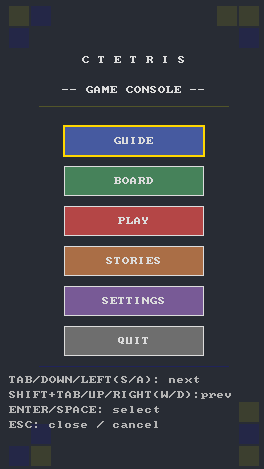
\includegraphics[width=0.3\textwidth]{09-gameConsoleGuide-screenshot-v2}
    \\[10pt]
    \textit{\small Hình 9.2: Màn hình module gameConsole - V2}
\end{figure}

\vspace{8pt}
\begin{center}
\begin{tikzpicture}[
    zone/.style={draw, rounded corners=3pt, minimum width=5.4cm, align=center,
                 font=\small},
    btn/.style={draw, rounded corners=2pt, minimum width=4.8cm,
                minimum height=0.52cm, align=center, font=\footnotesize}
]
    \draw[thick, rounded corners=6pt] (-0.2,-0.3) rectangle (5.6,8.2);
    \node[zone, fill=gray!15, minimum height=0.8cm] at (2.7,7.55)
        {\textbf{C TETRIS -- GAME CONSOLE}};
    \foreach \lbl/\col/\y in {
        GUIDE/blue!20/6.1,
        BOARD/green!25/5.45,
        PLAY/red!20/4.8,
        STORIES/orange!22/4.15,
        SETTINGS/violet!18/3.5,
        QUIT/gray!22/2.85
    }{
        \node[btn, fill=\col] at (2.7,\y) {\textbf{\lbl}};
    }
    \node[zone, fill=gray!8, minimum height=1.0cm] at (2.7,1.2)
        {{\footnotesize TAB / ENTER / ESC -- gợi ý phím tắt}};
    \node[font=\tiny\itshape, text=gray] at (0.55, 7.2) {silhouette};
    \node[font=\tiny\itshape, text=gray] at (4.85, 7.2) {silhouette};
    \node[font=\tiny\itshape, text=gray] at (0.55, 0.3) {silhouette};
    \node[font=\tiny\itshape, text=gray] at (4.85, 0.3) {silhouette};
\end{tikzpicture}
\end{center}
\vspace{4pt}

Màn hình chia \textbf{ba vùng} theo chiều dọc:

\vspace{4pt}
\begin{tabularx}{\linewidth}{|l|l|X|}
    \hline
    \textbf{Vùng}  & \textbf{Vị trí}        & \textbf{Nội dung} \\
    \hline
    Tiêu đề        & Trên cùng              & Tên thương hiệu \textit{C TETRIS -- GAME CONSOLE}. \\
    \hline
    Nút bấm        & Giữa (y=130--350)      & 6 nút 140$\times$30\,px, cách nhau 40\,px. \\
    \hline
    Phím tắt       & Dưới cùng              & Gợi ý TAB / ENTER / ESC cho người dùng mới. \\
    \hline
\end{tabularx}

\subsection{Hình nền -- tại sao không còn màu xám đơn điệu? (v2)}

V1 dùng màu trơn \texttt{\#282C34} làm nền -- thực dụng nhưng nhàm.
V2 thay bằng file SVG có \textbf{silhouette tetromino mờ 10\%} tại
bốn góc và \textbf{hai đường kẻ ngang} phân cách vùng tiêu đề và
vùng phím tắt.

\noindent\textbf{Kỹ thuật để bạn biết (không cần nhớ):}
\begin{itemize}
    \item SVG chỉ được vẽ \textbf{một lần} rồi lưu lại -- không vẽ lại mỗi frame.
    \item Khi quay lại gameConsole từ ván đấu, nền cũ bị xoá và vẽ mới --
          tránh dùng texture cũ từ phiên trước.
    \item Nếu vẽ thất bại (thiếu bộ nhớ), ứng dụng tự trở về nền xám cũ --
          không crash.
\end{itemize}

\subsection{Sáu nút điều khiển -- mỗi nút làm gì? (v2)}

\vspace{4pt}
\begin{tabularx}{\linewidth}{|c|l|l|X|}
    \hline
    \textbf{\#} & \textbf{Nút}     & \textbf{Màu}       & \textbf{Chức năng} \\
    \hline
    0 & \textbf{GUIDE}    & Xanh dương đậm & Mở hướng dẫn chơi -- nên xem trước khi vào. \\
    \hline
    1 & \textbf{BOARD}    & Xanh lá đậm   & Bảng xếp hạng -- ai điểm cao nhất. \\
    \hline
    2 & \textbf{PLAY}     & Đỏ đậm        & Bắt đầu ván đấu. Nếu đang chọn story,
                                            chạy dialogue trước rồi mới vào game. \\
    \hline
    3 & \textbf{STORIES}  & Cam đất       & Chọn tuyến truyện -- \textit{mới v2}. \\
    \hline
    4 & \textbf{SETTINGS} & Tím nhạt      & Âm lượng + màu khối -- \textit{mới v2}. \\
    \hline
    5 & \textbf{QUIT}     & Xám           & Thoát. Desktop: đóng cửa sổ.
                                            Web: màn hình Reload. \\
    \hline
\end{tabularx}

\notebox{Khi \textbf{bất kỳ popup nào đang mở}, toàn bộ 6 nút chính ẩn đi.
Muốn về màn hình chính: bấm ESC hoặc click \texttt{[X]} của popup trước.}

\subsection{Ba cách điều hướng -- dùng cái nào cũng được}

\subsubsection{Bàn phím}

\vspace{4pt}
\begin{tabularx}{\linewidth}{|l|X|}
    \hline
    \textbf{Phím}                                   & \textbf{Hành động} \\
    \hline
    \texttt{TAB} / \texttt{S} / \texttt{A}          & Focus tiến xuống nút kế tiếp. \\
    \hline
    \texttt{Shift+TAB} / \texttt{W} / \texttt{D}    & Focus lùi lên nút trước. \\
    \hline
    \texttt{ENTER} / \texttt{SPACE}                 & Kích hoạt nút đang focus. \\
    \hline
    \texttt{ESC}                                    & Nhảy focus về QUIT (hoặc đóng popup). \\
    \hline
\end{tabularx}

\tipbox{\texttt{ESC} không thoát app ngay -- nó chỉ \textit{focus} về nút QUIT.
Bạn vẫn phải bấm ENTER thêm lần nữa. Thiết kế này tránh thoát nhầm.}

\subsubsection{Chuột}

\begin{itemize}
    \item \textbf{Click chuột trái}: kích hoạt nút và cập nhật focus.
    \item \textbf{Click} \texttt{[X]}: đóng popup đang mở.
    \item \textbf{Con lăn chuột} (khi popup Guide / Board mở): cuộn nội dung.
\end{itemize}

\subsection{Scrollbar trong popup -- cuộn thế nào?}

\vspace{4pt}
\begin{tabularx}{\linewidth}{|l|X|}
    \hline
    \textbf{Cách cuộn}                         & \textbf{Mô tả} \\
    \hline
    Con lăn chuột                              & Cuộn theo chiều lăn -- nhanh nhất. \\
    \hline
    \texttt{W} / \texttt{$\uparrow$}           & Cuộn lên một dòng. \\
    \hline
    \texttt{S} / \texttt{$\downarrow$}         & Cuộn xuống một dòng. \\
    \hline
    Kéo thanh scrollbar                        & Drag chuột trực tiếp trên thanh. \\
    \hline
\end{tabularx}

\subsection{Popup BOARD -- bảng xếp hạng biết sắp xếp (v2)}

\begin{figure}[htbp]
    \centering
    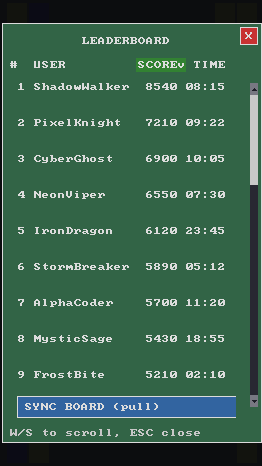
\includegraphics[width=0.3\textwidth]{09-gameConsoleGuide-screenshot-v2-board}
    \\[10pt]
    \textit{\small Hình 9.3: Màn hình module gameConsole - V2 - board popup}
\end{figure}

Từ v2, Board đọc dữ liệu thực từ SQLite và có thể sắp xếp theo
\textbf{4 chế độ}. Click nút \textbf{SCORE} hay \textbf{TIME} để chuyển;
click lần hai để đảo chiều. Nút đang active có nền xanh lá đậm.

\vspace{4pt}
\begin{tabularx}{\linewidth}{|l|l|X|}
    \hline
    \textbf{Nút}                    & \textbf{Chế độ}      & \textbf{Ý nghĩa} \\
    \hline
    \textbf{SCORE\,$\downarrow$}    & \texttt{SCORE\_DESC} & Điểm cao nhất trước -- \textit{mặc định}. \\
    \hline
    \textbf{SCORE\,$\uparrow$}      & \texttt{SCORE\_ASC}  & Điểm thấp nhất trước. \\
    \hline
    \textbf{TIME\,$\downarrow$}     & \texttt{TIME\_DESC}  & Bản ghi mới nhất trước. \\
    \hline
    \textbf{TIME\,$\uparrow$}       & \texttt{TIME\_ASC}   & Bản ghi cũ nhất trước. \\
    \hline
\end{tabularx}

\noindent Điểm của bạn được \textbf{lưu tự động} sau mỗi ván kể từ v2.

\subsection{Popup STORIES -- chọn câu chuyện trước khi chơi (v2)}

\begin{figure}[htbp]
    \centering
    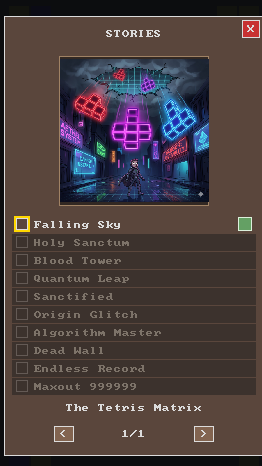
\includegraphics[width=0.3\textwidth]{09-gameConsoleGuide-screenshot-v2-stories}
    \\[10pt]
    \textit{\small Hình 9.4: Màn hình module gameConsole - v2 - stories popup}
\end{figure}

Mỗi story là tuyến truyện kèm cài đặt ván đấu riêng. Chọn story $\Rightarrow$
ván đấu tiếp theo theo cài đặt đó.

\vspace{4pt}
\begin{tabularx}{\linewidth}{|l|l|X|}
    \hline
    \textbf{Trạng thái} & \textbf{Nhìn vào}        & \textbf{Ý nghĩa} \\
    \hline
    Locked              & Radio mờ / icon khoá     & Chưa đủ điều kiện mở khoá. \\
    \hline
    Unlocked            & Radio chọn được          & Có thể chọn và chơi. \\
    \hline
    Selected            & Radio đặc (tô đầy)      & Story đang được chọn cho ván tới. \\
    \hline
\end{tabularx}

\vspace{4pt}
\noindent\textbf{Thao tác trong popup Stories:}

\vspace{4pt}
\begin{tabularx}{\linewidth}{|l|X|}
    \hline
    \textbf{Hành động}                    & \textbf{Kết quả} \\
    \hline
    Click radio / tên story               & Chọn story (cập nhật DB, popup vẫn mở). \\
    \hline
    Click \textbf{Play}                   & Chọn + đóng popup + chạy dialogue. \\
    \hline
    Click $\leftarrow$ / $\rightarrow$    & Chuyển chapter, tải lại danh sách từ DB. \\
    \hline
    \texttt{ESC} / click \texttt{[X]}     & Đóng popup -- lựa chọn được giữ nguyên. \\
    \hline
\end{tabularx}

\subsection{Popup SETTINGS -- tinh chỉnh trải nghiệm (v2)}

\begin{figure}[htbp]
    \centering
    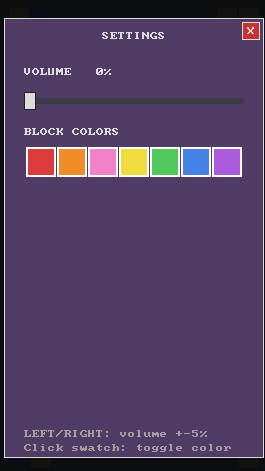
\includegraphics[width=0.3\textwidth]{09-gameConsoleGuide-screenshot-v2-setting}
    \\[10pt]
    \textit{\small Hình 9.5: Màn hình module gameConsole - v2 - setting popup}
\end{figure}

\noindent\textbf{Hai cài đặt:}

\begin{enumerate}
    \item \textbf{Âm lượng} -- slider 0\%--100\%. Phím \texttt{LEFT}/\texttt{RIGHT}
          điều chỉnh mỗi bước 5\%. Thay đổi có hiệu lực ngay lập tức.

    \item \textbf{Màu khối} -- 7 checkbox: Đỏ, Cam, Hồng, Vàng, Xanh lá, Xanh
          dương, Tím. Màu nào được bật mới xuất hiện trong ván. Ít nhất 1 màu
          phải bật -- ứng dụng không để bạn tắt hết.
\end{enumerate}

\notebox{Cài đặt được \textbf{lưu ngay khi đóng popup} (ESC hoặc click X).
Lần sau mở app, cài đặt cũ vẫn còn đó.}

\vspace{4pt}
\begin{tabularx}{\linewidth}{|l|X|}
    \hline
    \textbf{Thao tác}                      & \textbf{Kết quả} \\
    \hline
    \texttt{LEFT} / \texttt{RIGHT}         & Giảm / tăng âm lượng 5\%. \\
    \hline
    Click checkbox màu                     & Bật / tắt màu đó. \\
    \hline
    \texttt{ESC} / click \texttt{[X]}      & Đóng popup \textbf{và lưu} vào DB. \\
    \hline
\end{tabularx}

\subsection{Nhạc nền -- nghe thấy không?}

Khi vào gameConsole, stream âm thanh đã mở và volume control thực sự
hoạt động. Tuy nhiên, \textbf{chưa có file nhạc được nạp vào} nên bạn
không nghe thấy gì. Kiến trúc đã sẵn sàng -- chờ V3 nạp file nhạc.

\subsection{Màn hình Reload -- chỉ trên trình duyệt web}

\begin{figure}[htbp]
    \centering
    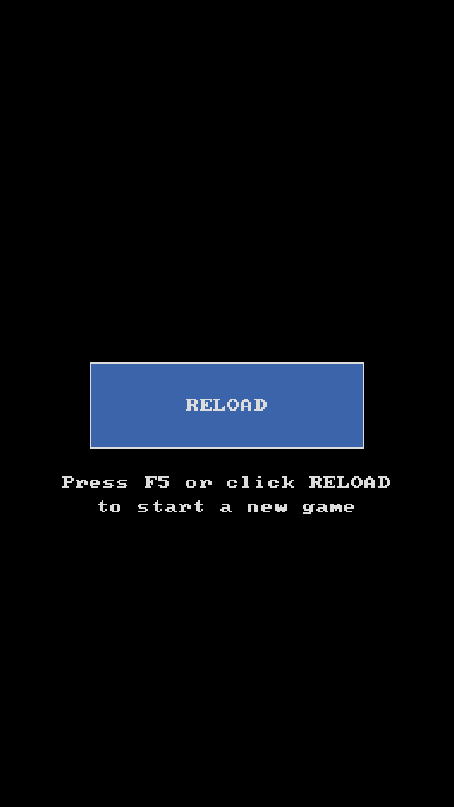
\includegraphics[width=0.3\textwidth]{09-gameConsoleGuide-screenshot-v2-reload}
    \\[10pt]
    \textit{\small Hình 9.6: Màn hình module gameConsole - v2 - reload}
\end{figure}

Bấm \textbf{QUIT} trên Web không đóng tab được -- ứng dụng hiện màn hình
này thay. Tải lại bằng: click \textbf{RELOAD}, hoặc nhấn \texttt{F5} /
\texttt{ENTER} / \texttt{SPACE}.

\vspace{4pt}
\begin{tabularx}{\linewidth}{|l|X|}
    \hline
    \textbf{Nền tảng}    & \textbf{Nhấn QUIT thì xảy ra gì} \\
    \hline
    Desktop (native)     & Đóng cửa sổ ngay lập tức. \\
    \hline
    Web (WASM)           & Màn hình đen + nút RELOAD lớn. \\
    \hline
\end{tabularx}

\subsection{Tổng hợp phím tắt -- tra cứu nhanh}

\subsubsection{Màn hình chính}
\begin{tabularx}{\linewidth}{|l|X|}
    \hline
    \textbf{Phím}                                & \textbf{Hành động} \\
    \hline
    \texttt{TAB} / \texttt{S} / \texttt{A}       & Focus tiến tới nút kế tiếp. \\
    \hline
    \texttt{Shift+TAB} / \texttt{W} / \texttt{D} & Focus lùi về nút trước. \\
    \hline
    \texttt{ENTER} / \texttt{SPACE}              & Kích hoạt nút đang focus. \\
    \hline
    \texttt{ESC}                                 & Nhảy focus về nút QUIT. \\
    \hline
\end{tabularx}

\subsubsection{Khi popup Guide hoặc Board đang mở}
\begin{tabularx}{\linewidth}{|l|X|}
    \hline
    \textbf{Phím / Hành động}          & \textbf{Kết quả} \\
    \hline
    \texttt{W} / \texttt{$\uparrow$}   & Cuộn lên. \\
    \hline
    \texttt{S} / \texttt{$\downarrow$} & Cuộn xuống. \\
    \hline
    Con lăn chuột                      & Cuộn theo chiều lăn. \\
    \hline
    \texttt{ESC} / click \texttt{[X]}  & Đóng popup. \\
    \hline
\end{tabularx}

\subsubsection{Khi popup Settings đang mở}
\begin{tabularx}{\linewidth}{|l|X|}
    \hline
    \textbf{Phím / Hành động}          & \textbf{Kết quả} \\
    \hline
    \texttt{LEFT} / \texttt{RIGHT}     & Giảm / tăng âm lượng 5\%. \\
    \hline
    \texttt{ESC} / click \texttt{[X]}  & Đóng \textbf{và lưu} cài đặt. \\
    \hline
\end{tabularx}

\subsubsection{Khi popup Stories đang mở}
\begin{tabularx}{\linewidth}{|l|X|}
    \hline
    \textbf{Hành động}                        & \textbf{Kết quả} \\
    \hline
    Click radio / tên story                   & Chọn story, cập nhật DB. \\
    \hline
    Click \textbf{Play}                       & Chọn + đóng + chạy dialogue. \\
    \hline
    Click $\leftarrow$ / $\rightarrow$        & Chuyển chapter. \\
    \hline
    \texttt{ESC} / click \texttt{[X]}         & Đóng (không mất lựa chọn). \\
    \hline
\end{tabularx}

\subsection{Còn thiếu gì -- và khi nào có?}

\vspace{4pt}
\begin{tabularx}{\linewidth}{|l|l|X|}
    \hline
    \textbf{Tính năng}         & \textbf{Hiện tại (v2)} & \textbf{Dự kiến} \\
    \hline
    Board đồng bộ cloud        & Local SQLite           & V3: Cloudflare D1 Worker. \\
    \hline
    Đăng ký tham gia board         & Chưa có                & V3: email + OTP. \\
    \hline
    Nhạc nền thực sự           & Stub (gain hoạt động)  & V3: nạp file nhạc. \\
    \hline
    Thumbnail Stories popup    & Placeholder            & V3: load từ đường dẫn. \\
    \hline
\end{tabularx}

\label{LastPageGameConsoleGuide}
\end{document}




